\documentclass{beamer}
\usepackage{listings}
\usepackage{color}
\usepackage{graphics}

\lstset{
  language=Ruby
}

\begin{document}
\title{Welcome to Elixir}
\subtitle{
  \textit{
    \linebreak
    ``This is good shit``
    \linebreak
  }
  \tiny{\textrm{--- Joe Armstrong}}
}
\frame{\titlepage}

\AtBeginSection[]{
  \begin{frame}
    \frametitle{Table of Contents}
    \tableofcontents[currentsection]
  \end{frame}
}

\section[Section]{Overview}

\begin{frame}
  \frametitle{Motivation}
  \begin{itemize}
  \item Power of Erland
  \item Elixir basics
  \item Macros
  \item Tooling and abstractions
  \end{itemize}
\end{frame}

\section[Section]{Power of Erland}

\begin{frame}
  \frametitle{Erlang}
  \begin{itemize}
  \item created in mid-1980s
  \item designed for telecom
  \item connect multiple systems
  \item minimal impact of errors
  \item entire system should never go down
  \end{itemize}
\end{frame}

\begin{frame}
  \frametitle{High availability}
  \begin{itemize}
  \item fault tolerance
  \item scalability
  \item distribution
  \item responsiveness
  \item live update
  \end{itemize}
\end{frame}

\begin{frame}
  \frametitle{How do they do it?}
  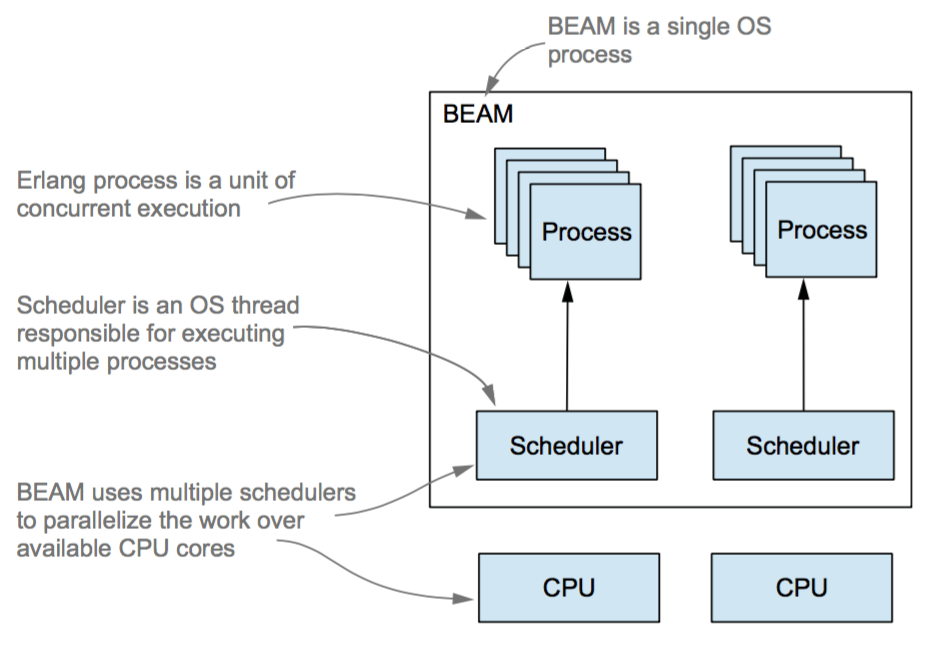
\includegraphics[scale=.5]{beam.png}
\end{frame}

\section[Section]{Elixir basics}

\begin{frame}
  \frametitle{Syntax}
  ``Elixir syntax is like a marriage of DSL
  friendly Ruby and the powerful hygenic macros of Clojure.``
  \linebreak
  \textrm{-- Devin Torres}
\end{frame}

\begin{frame}[fragile]
  \frametitle{The basics you know}
  \begin{lstlisting}
    1 + 1           # => 2
    2 * (3 + 1) / 4 # => 2.0
    1 + 2; 1 + 3    # => 4

    greeting = "Hello World!"
    IO.puts(greeting)
    # => Hello World!
    # => :ok
  \end{lstlisting}
\end{frame}

\begin{frame}[fragile]
  \frametitle{Modules and function, oh my!}
  \begin{lstlisting}
    defmodule Geometry do
      def rectangle_area(a, b) do
        a * b
      end
    end
  \end{lstlisting}
\end{frame}

\begin{frame}[fragile]
  \frametitle{Composing functions}
  \begin{lstlisting}
    def process_xml(model, xml) do
      model
      |> update(xml)
      |> process_changes
      |> persist
    end
  \end{lstlisting}
\end{frame}

\begin{frame}[fragile]
  \frametitle{Function arity}
  \begin{lstlisting}
    defmodule Rectangle do
      def area(a), do: area(a, a)
      def area(a, b), do: a * b
    end
  \end{lstlisting}
\end{frame}

\begin{frame}[fragile]
  \frametitle{Typespec}
  \begin{lstlisting}
    % read up on dializer and custom types
    defmodule Circle do
      @pi 3.14159

      @spec area(number) :: number
      def area(r), do: r*r*@pi
        
      @spec circumference(number) :: number
      def circumference(r), do: 2*r*@pi
    end
  \end{lstlisting}
\end{frame}

\section[Section]{Macros}

\section[Section]{Tooling and Abstractions}
  
\end{document}
